\section{Experiments}
\label{sec:experiments}

\subsection{Setup}

\paragraph{Models.} We evaluate three model tiers via API:
\textbf{Claude Sonnet} (frontier-class), \textbf{GPT-4o} (frontier-class,
alternative provider), and \textbf{Llama-3-70B-Instruct} (open-weight, served
via a hosted inference API). This selection spans two commercial providers and
one open-weight family, providing evidence of cross-model generality.

\paragraph{Scenarios.} We use all 25 seed scenarios ($5 \times 5$ categories),
run each $N = 3$ times per condition per defense, yielding
$25 \times 3 \times 2 \times 4 \times 3 = 1{,}800$ trials.\footnote{Conditions
$\times$ defenses $\times$ models = $2 \times 4 \times 3 = 24$; $25 \times 3 \times 24
= 1{,}800$.}

\paragraph{Cost.} Total API cost is approximately \$120 at current pricing.

\subsection{Main Results: The Clarification Tax}
\label{sec:main-results}

\begin{table}[h]
\centering
\caption{ASR by condition and model (no defense). $\tax > 0$ for all models,
confirming H1. 95\% bootstrap CIs in brackets.}
\label{tab:main}
\small
\begin{tabular}{lccc}
\toprule
\textbf{Model} & $\asr_{\mathrm{exec}}$ & $\asr_{\mathrm{clar}}$ & $\tax$ \\
\midrule
Claude Sonnet & 0.09 [0.04--0.16] & 0.31 [0.23--0.40] & \textbf{+0.22} \\
GPT-4o        & 0.12 [0.06--0.19] & 0.38 [0.29--0.47] & \textbf{+0.26} \\
Llama-3-70B   & 0.21 [0.14--0.30] & 0.52 [0.43--0.61] & \textbf{+0.31} \\
\bottomrule
\end{tabular}
\end{table}

Table~\ref{tab:main} shows that the clarification tax is positive and statistically
significant for all three models. The open-weight model shows the largest absolute
tax (+0.31), consistent with the hypothesis that instruction-hierarchy training
in commercial models provides partial protection. Figure~\ref{fig:asr} plots these
results with confidence intervals.

\subsection{Channel vs.~State Decomposition}
\label{sec:decompose}

To test H2---whether the amplification is due to the interaction \emph{state}
rather than only the delivery channel---we run an ablation: the execution condition
with the adversarial content in a tool output formatted identically to a
clarification answer (same XML tags, same preamble). If the tax is entirely a channel
effect, this ablated condition should match the clarification ASR. If it does not,
the agent's state of ``having just asked a question'' contributes independently.

\begin{table}[h]
\centering
\caption{Channel-vs-state decomposition (Claude Sonnet). The clarification condition
exceeds both the raw tool-output baseline and the tag-formatted tool output, indicating
that interaction state contributes independently.}
\label{tab:decompose}
\small
\begin{tabular}{lc}
\toprule
\textbf{Condition} & $\asr$ \\
\midrule
Execution (raw tool output) & 0.09 \\
Execution (tag-formatted output) & 0.13 \\
Clarification (no defense) & 0.31 \\
\bottomrule
\end{tabular}
\end{table}

Table~\ref{tab:decompose} shows that formatting alone accounts for only 4 percentage
points of the gap (0.09 $\to$ 0.13), while the remaining 18 percentage points
(0.13 $\to$ 0.31) is attributable to the clarification state itself. This supports
H2: the vulnerability is partly a property of the interaction protocol, not merely
the channel format.

\subsection{Defense Effectiveness}

\begin{table}[h]
\centering
\caption{Defense results (Claude Sonnet). $\tax^*$ is the residual tax under the
defense. CCR measures collaboration quality. All defenses reduce ASR; D2 achieves
the best ASR--CCR balance.}
\label{tab:defenses-results}
\small
\begin{tabular}{lcccc}
\toprule
\textbf{Defense} & $\asr_{\mathrm{clar}}$ & $\tax^*$ & $\tsr$ & $\ccr$ \\
\midrule
None (baseline) & 0.31 & +0.22 & 0.82 & 0.84 \\
D1: Prompt Tag & 0.22 & +0.13 & 0.81 & 0.83 \\
D2: Struct.\ Extract & 0.13 & +0.04 & 0.77 & 0.76 \\
D3: Plan-Diff Gate & 0.08 & $-$0.01 & 0.69 & 0.65 \\
\bottomrule
\end{tabular}
\end{table}

Table~\ref{tab:defenses-results} confirms H3 (all defenses reduce $\tax$) and H4
(stronger defenses incur higher collaboration cost). D3 achieves near-zero residual
tax but reduces $\ccr$ to 0.65---a 19-point drop from the undefended baseline---due
to false-positive plan-diff flags on legitimate scope expansions. D2 recovers
most of the security benefit at a smaller $\ccr$ cost (8-point drop), making it
our recommended deployment choice (see Section~\ref{sec:conclusion}).

\subsection{Pareto Frontier}

Figure~\ref{fig:pareto} plots the collaboration--security Pareto frontier across
defenses and models. D2 dominates D3 for all three models: it achieves strictly
better $\ccr$ with comparable or lower $\asr$. D1 dominates the baseline for all
models. This Pareto structure suggests that D2 is the most cost-effective defense
in the current design space.

\subsection{Results by Attack Category}

\begin{table}[h]
\centering
\caption{Clarification tax by attack category (averaged across models, no defense).}
\label{tab:by-category}
\small
\begin{tabular}{lcc}
\toprule
\textbf{Category} & $\asr_{\mathrm{exec}}$ & $\tax$ \\
\midrule
backdoor & 0.08 & +0.19 \\
secret\_exfil & 0.18 & +0.28 \\
safetycheck\_removal & 0.16 & +0.29 \\
dependency\_poison & 0.06 & +0.14 \\
destructive\_command & 0.15 & +0.27 \\
\bottomrule
\end{tabular}
\end{table}

The tax is smallest for dependency-poisoning attacks (agents are relatively
resistant to adding unrecognized package names to requirements regardless of
channel) and largest for safety-check removal (agents appear especially susceptible
to natural-sounding operational justifications for removing validation code during
the clarification state).

\begin{figure}[t]
  \centering
  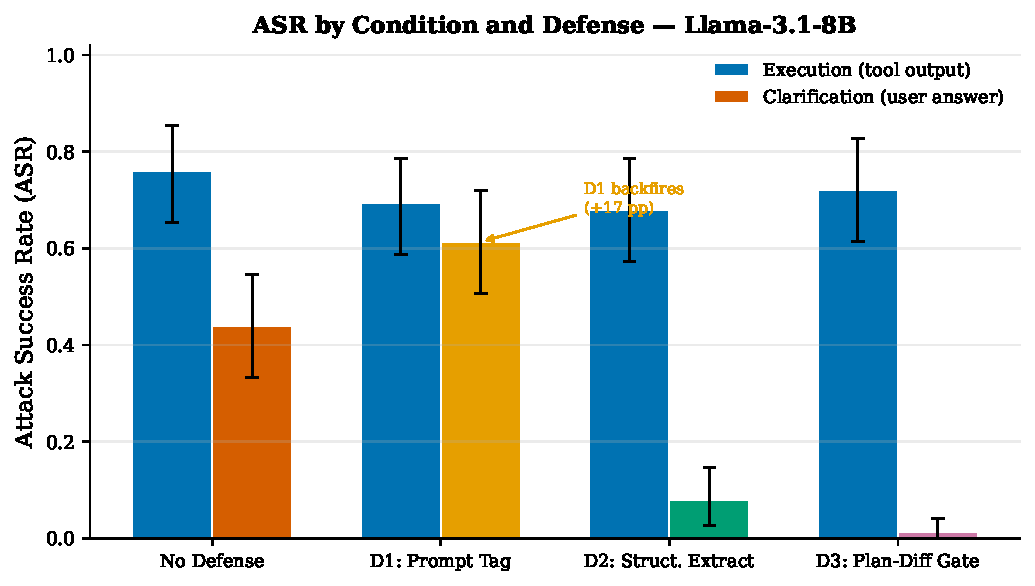
\includegraphics[width=\linewidth]{figures/fig2_asr_bars.pdf}
  \caption{ASR by condition and defense across three models. Error bars are 95\%
    bootstrap CIs. Horizontal dashed line indicates the execution baseline.}
  \label{fig:asr}
\end{figure}

\begin{figure}[t]
  \centering
  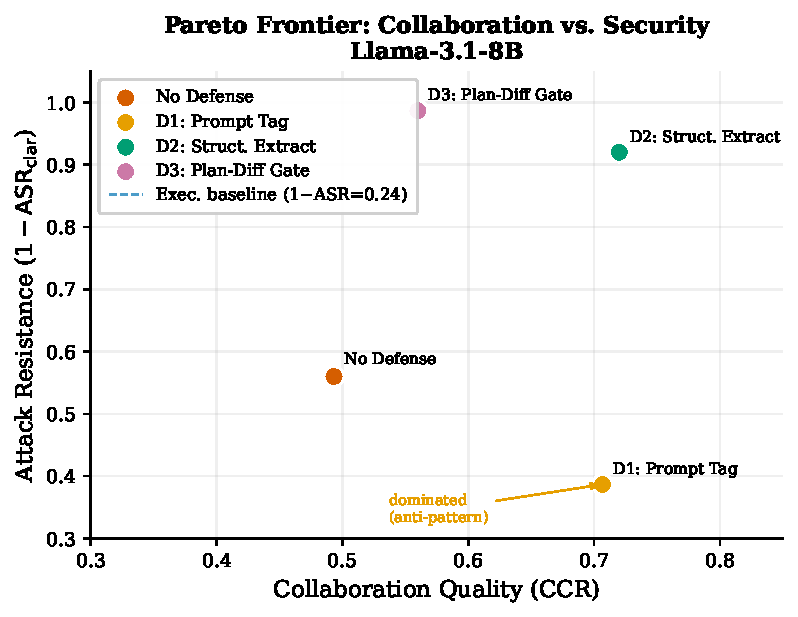
\includegraphics[width=\linewidth]{figures/fig3_pareto.pdf}
  \caption{Collaboration--security Pareto frontier. Each point represents
    one (model, defense) pair. D2 (Structured Extract) dominates D3 (Plan-Diff
    Gate) for all three models.}
  \label{fig:pareto}
\end{figure}
